%%
%% Author: Moritz
%% 18.03.2018
%%

% Preamble
\documentclass[../../Pflichtenheft.tex]{subfiles}
\begin{document}
    \subsection{Aufenthalt}
    \begin{figure}[ht!]
        \begin{center}
            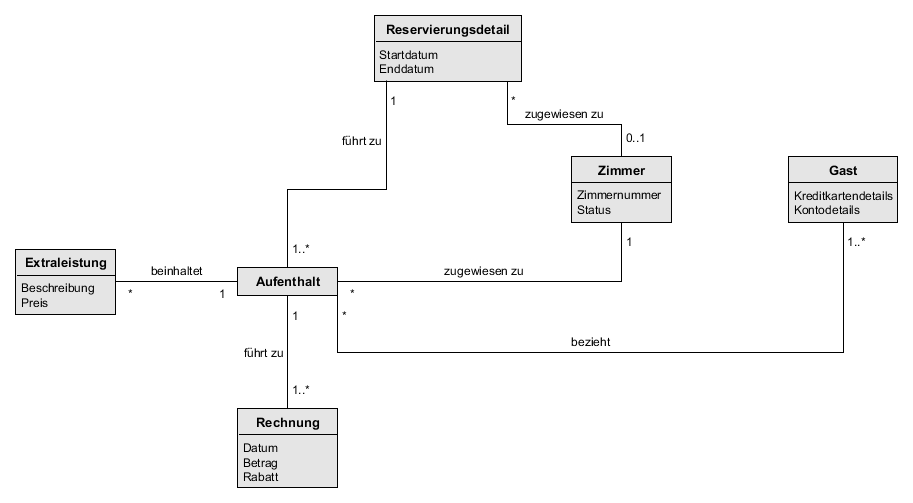
\includegraphics[width=0.5\linewidth]{assets/aufenthalt.png}
            \caption{Objekt 'Aufenthalt'} \label{aufenthalt_model}
        \end{center}
    \end{figure}
    Ein Aufenthalt dient zur Überführung einer Reservierung in den tatsächlichen Aufenthalt eines
    Gastes, welcher beim Check-In entsteht. Dies führt gründsätzlich zur Erstellung eines Rechnungsbjektes.
    Zudem können zum Aufenthalt Extraleistungen gebucht werden, die aber erst während dem
    Aufenthalt anfallen und aus diesem Grund auch noch nicht mit den Resvierungsdetails verknüpft sind.
    \\Des weiteren wird zum Aufenthalt ein Gast zugeteilt, der den Aufenthalt dann auch tatsächlich wahrnimmt.
    Zu jedem Aufenthalt wird zudem ein Zimmer zugeordnet. Dies kann manuell oder automatisch vom System vorgenommen
    werden.
\end{document}